\documentclass{../../../kin_math}

\header{Elijah Kin}{Homework 3}{AMSC660}
\headrule

\begin{document}

\begin{questions}
  \question \emph{Additional reading for this problem: \href{https://www.stat.uchicago.edu/~lekheng/courses/302/demmel/}{J. Demmel, Applied Numerical Linear Algebra}, available online via the UMCP library.}

  The goal of this exercise is to understand how one can compute a QR decomposition using \emph{Householder reflections}.
  \begin{enumerate}
    \item Let $u$ be a unit vector in $\mathbb{R}^n$, i.e., $\lVert u \rVert_2 = 1$. Let $P = I - 2uu^\top$. This matrix performs reflection with respect to the hyperplane orthogonal to the vector $u$. Show that $P = P^\top$ and $P^2 = I$.
    \begin{solution}
      By the definition of $P$ and the linearity of transpose,
      \begin{equation*}
        P^\top = (I - 2uu^\top)^\top = I^\top - 2(uu^\top)^\top.
      \end{equation*}
      But then since $I^\top = I$ and $(uu^\top)^\top = (u^\top)^\top u^\top = uu^\top$,
      \begin{equation*}
        P^\top = I^\top - 2(uu^\top)^\top = I - 2uu^\top = P
      \end{equation*}
      and hence $P = P^\top$ as desired.

      Now observe that since $I^2 = I$ and $I(uu^\top) = (uu^\top)I = uu^\top$,
      \begin{equation*}
        P^2 = (I - 2uu^\top)(I - 2uu^\top) = I - 4uu^\top + 4(uu^\top)^2.
      \end{equation*}
      But then because $\lVert u \rVert_2 = 1$,
      \begin{equation*}
        (uu^\top)^2 = u(u^\top u)u^\top = u\lVert u \rVert_2 u^\top = uu^\top
      \end{equation*}
      and hence
      \begin{equation*}
        P^2 = I - 4uu^\top + 4(uu^\top)^2 = I - 4uu^\top + 4uu^\top = I.
      \end{equation*}
    \end{solution}
    \item Let $x \in \mathbb{R}^n$ be any vector, $x = \begin{bmatrix} x_1, \dots, x_n \end{bmatrix}^\top$. Let $u$ be defined as follows:
    \begin{equation} \label{house}
      \tilde{u} \coloneqq \begin{bmatrix} x_1 + \textsf{sign}(x_1) \lVert x \rVert_2 \\ x_2 \\ \vdots \\ x_n \end{bmatrix} \equiv x + \textsf{sign}(x_1) \lVert x \rVert_2 e_1, \quad u = \frac{\tilde{u}}{\lVert \tilde{u} \rVert_2},
    \end{equation}
    where $e_1 = \begin{bmatrix} 1, 0, \dots, 0 \end{bmatrix}^\top$. The matrix with the vector $u$ constructed according to (\ref{house}) will be denoted $\textsf{House}(x)$:
    \begin{equation*}
      P = I - 2uu^\top \equiv I - 2\frac{\tilde{u}\tilde{u}^\top}{\tilde{u}^\top\tilde{u}} \equiv \textsf{House}(x).
    \end{equation*}
    Calculate $Px$.
    \begin{solution}
      We claim first that $2 \tilde{u}^\top x = \tilde{u}^\top \tilde{u}$. To see this, note that
      \begin{multline*}
        2 \tilde{u}^\top x = 2 (x + \textsf{sign}(x_1) \lVert x \rVert_2 e_1)^\top x = 2 (x^\top + \textsf{sign}(x_1) \lVert x \rVert_2 e_1^\top) x \\
        = 2 x^\top x + 2 \textsf{sign}(x_1) \lVert x \rVert_2 e_1^\top x = 2 x^\top x + 2 \textsf{sign}(x_1) \lVert x \rVert_2 x_1 = 2 x^\top x + 2 |x_1| \lVert x \rVert_2
      \end{multline*}
      and also that since $x^\top e_1 = e_1^\top x = x_1$ and $e_1^\top e_1 = 1$ and $\textsf{sign}(x_1)^2 = 1$,
      \begin{multline*}
        \tilde{u}^\top \tilde{u} = (x + \textsf{sign}(x_1) \lVert x \rVert_2 e_1)^\top (x + \textsf{sign}(x_1) \lVert x \rVert_2 e_1) \\
        = (x^\top + \textsf{sign}(x_1) \lVert x \rVert_2 e_1^\top) (x + \textsf{sign}(x_1) \lVert x \rVert_2 e_1) = x^\top x + 2 \textsf{sign}(x_1) \lVert x \rVert_2 x_1 + \lVert x \rVert_2^2 \\
        = x^\top x + 2 |x_1| \lVert x \rVert_2 + x^\top x = 2x^\top x + 2 |x_1| \lVert x \rVert_2
      \end{multline*}
      Hence, we have that $2 \tilde{u}^\top x = \tilde{u}^\top \tilde{u}$ (notably a scalar quantity). Then it follows that
      \begin{equation*}
        2 \frac{\tilde{u} \tilde{u}^\top}{\tilde{u}^\top \tilde{u}} x = \tilde{u} \cdot \frac{2 \tilde{u}^\top x}{\tilde{u}^\top \tilde{u}} = \tilde{u}
      \end{equation*}
      and so
      \begin{equation*}
        Px = \left(I - 2 \frac{\tilde{u} \tilde{u}^\top}{\tilde{u}^\top \tilde{u}}\right)x = x - 2 \frac{\tilde{u} \tilde{u}^\top}{\tilde{u}^\top \tilde{u}}x = x - \tilde{u} = -\textsf{sign}(x_1) \lVert x \rVert_2 e_1.
      \end{equation*}
    \end{solution}
    \item Let $A$ be an $m \times n$ matrix, $m \geq n$, with columns $a_j$, $j = 1, \dots, n$. Let $A_0 = A$. Let $P_1 = \textsf{House}(a_1)$. Then $A_1 \coloneqq P_1A_0$ has the first column with the first entry nonzero and the other entries being zero. Next, we define $P_2$ as
    \begin{equation*}
      P_2 = \begin{bmatrix} 1 & 0 \\ 0 & \tilde{P}_2 \end{bmatrix}
    \end{equation*}
    where the matrix $\tilde{P}_2 = \textsf{House}(A_1(2 : m, 2))$. The notation $A_1(2 : m, 2)$ is Matlab's syntax indicating this is the vector formed by entries 2 through $m$ of the 2nd column of $A_1$. Then we set $A_2 = P_2A_1$. And so on.

    This algorithm can be described as follows. Let $A_0 = A$. Then for $j = 1, 2, \dots, n$ we set
    \begin{equation*}
      P_j = \begin{bmatrix} I_{(j - 1) \times (j - 1)} & 0 \\ 0 & \tilde{P}_j \end{bmatrix}; \quad \tilde{P}_j = \textsf{House}(A_{j - 1}(j : m, j)), \quad A_j = P_jA_{j - 1}.
    \end{equation*}
    Check that the resulting matrix $A_n$ is upper triangular, its entries $(A_n)_{ij}$ are all zeros for $i > j$. Propose an \texttt{if}-statement in this algorithm that will guarantee that $A_n$ has positive entries $(A_n)_{jj}$, $1 \leq j \leq n$.
    \begin{solution}
      We proceed by induction on $k$ to show that for $0 \leq k \leq n$, $A_k$ is upper triangular in columns $1 \leq j \leq k$. The base case of $k = 0$ is trivially true, since the hypothesis asserts nothing about $A_0$; there are no columns $1 \leq j \leq 0$.

      Now for some $0 \leq k \leq n - 1$, suppose $A_k$ is upper triangular in columns $1 \leq j \leq k$. Further, note that the entry
      \begin{multline*}
        (A_{k + 1})_{ij} = (P_{k + 1} A_k)_{ij} = \sum_{\ell = 1}^m (P_{k + 1})_{i \ell} (A_k)_{\ell j} \\
        = \sum_{\ell = 1}^k (P_{k + 1})_{i \ell} (A_k)_{\ell j} + \sum_{\ell = k + 1}^m (P_{k + 1})_{i \ell} (A_k)_{\ell j}.
      \end{multline*}
      Further, recall that by definition,
      \begin{equation*}
        P_{k + 1} = \begin{bmatrix} I_{k \times k} & 0 \\ 0 & \tilde{P}_{k + 1} \end{bmatrix}
      \end{equation*}
      and so it follows that
      \begin{equation}
        \label{eq:pcase}
        (P_{k + 1})_{i \ell} = \begin{cases} (\tilde{P}_{k + 1})_{i - k, \ell - k} & i, \ell > k \\ 1 & i = \ell \leq k \\ 0 & \text{otherwise} \end{cases}.
      \end{equation}
      Now focusing first on the left summation, note that because $A_k$ is upper triangular in columns $1 \leq j \leq k$, and the first case of (\ref{eq:pcase}) is not possible since $\ell \leq k$, we have that
      \begin{equation*}
        \sum_{\ell = 1}^k (P_{k + 1})_{i \ell} (A_k)_{\ell j} = \sum_{\ell = 1}^j (P_{k + 1})_{i \ell} (A_k)_{\ell j} = \sum_{\ell = 1}^j (A_k)_{\ell j} \begin{cases} 1 & i = \ell \\ 0 & i \neq \ell \end{cases} = \begin{cases} (A_k)_{ij} & i \leq j \\ 0 & i > j \end{cases}.
      \end{equation*}
      We now focus on the right summation, in which the second case of (\ref{eq:pcase}) is not possible since $\ell > k$. Then
      \begin{multline*}
        \sum_{\ell = k + 1}^m (P_{k + 1})_{i \ell} (A_k)_{\ell j} = \sum_{\ell = k + 1}^m (A_k)_{\ell j} \begin{cases} 0 & i \leq k \\ (\tilde{P}_{k + 1})_{i - k, \ell - k} & i > k \end{cases} \\
        = \begin{cases} 0 & i \leq k \\ \sum_{\ell = k + 1}^m (\tilde{P}_{k + 1})_{i - k, \ell - k} (A_k)_{\ell j} & i > k \end{cases}
      \end{multline*}
      and hence
      \begin{equation*}
        (A_{k + 1})_{ij} = \begin{cases} (A_k)_{ij} & i \leq j \\ 0 & i > j \end{cases} + \begin{cases} 0 & i \leq k \\ \sum_{\ell = k + 1}^m (\tilde{P}_{k + 1})_{i - k, \ell - k} (A_k)_{\ell j} & i > k \end{cases}.
      \end{equation*}
      From the above, note that for $1 \leq j \leq k$, if $i > j$ then both summands will be 0 (the right will be 0 because $\ell > k \geq j$ so $(A_k)_{\ell j} = 0$ since $j \leq k$). Hence, it suffices to show that $A_{k + 1}$ is upper triangular in column $j = k + 1$;

      The left summand cannot contribute any nonzero values if $i > j$, so we need only consider the right summand. Re-indexing to write it as a matrix multiplication using the Matlab notation and taking $j = k + 1$,
      \begin{multline*}
        \sum_{\ell = k + 1}^m (\tilde{P}_{k + 1})_{i - k, \ell - k} (A_k)_{\ell j} = \sum_{\ell = 1}^{m - k} (\tilde{P}_{k + 1})_{i - k, \ell} (A_k)_{k + \ell, j} \\
        = (\tilde{P}_{k + 1} A_k(k + 1 : m, j))_{i - k} = (\tilde{P}_{k + 1} A_k(k + 1 : m, k + 1))_{i - k}.
      \end{multline*}
      But then by item (b),
      \begin{multline*}
        (\tilde{P}_{k + 1} A_k(k + 1 : m, k + 1))_{i - k} = (-\textsf{sign}((A_k)_{k + 1, k + 1}) \lVert A_k(k + 1 : m, k + 1) \rVert_2 e_1)_{i - k} \\
        = -\textsf{sign}((A_k)_{k + 1, k + 1}) \lVert A_k(k + 1 : m, k + 1) \rVert_2 (e_1)_{i - k}
      \end{multline*}
      which is $0$ if $i > j = k + 1$ since then $i - k \geq 2$ so $(e_1)_{i - k} = 0$. Hence, we have that $A_{k + 1}$ is upper triangular in columns $1 \leq j \leq k + 1$, so by the principle of induction, for any $0 \leq k \leq n$, $A_k$ is upper triangular in columns $1 \leq j \leq k$. Letting $k = n$, we obtain the desired result: $A_n$ is upper triangular in columns $1 \leq j \leq n$.

      If we want to ensure that the diagonal entries $(A_n)_{jj} \geq 0$ for $1 \leq j \leq n$, we could alter the definition of $\tilde{u}$ such that
      \begin{equation*}
        \tilde{u} \equiv x + \frac{|x_1|}{x_1} \lVert x \rVert_2 e_1,
      \end{equation*}
      that is, if $A_jj < 0$ then use $\tilde{u}  = x - \textsf{sign}(x_1) \lVert x \rVert_2 e_1$.
    \end{solution}
    \item Extract the QR decomposition of $A$ given the matrices $P_j$, $1 \leq j \leq n$, and $A_n$.
    \begin{solution}
      From (c) we know that $A_n$ is upper triangular. Hence, it suffices to construct an orthogonal matrix $Q$ from the matrices $P_j$, $1 \leq j \leq n$ such that $A = QA_n$.

      Towards this end, note that
      \begin{equation*}
        A_n = P_n A_{n - 1} = P_n P_{n - 1} A_{n - 2} = \dots = P_n P_{n - 1} \dots P_1 A_0 = P_n P_{n - 1} \dots P_1 A
      \end{equation*}
      so $Q$ should be defined such that
      \begin{equation*}
        A = Q P_n P_{n - 1} \dots P_1 A
      \end{equation*}
      and so
      \begin{equation*}
        Q = P_1^{-1} P_2^{-1} \dots P_n^{-1}.
      \end{equation*}
      But finally, from (a) we know that each $P_j$ is orthogonal ($P_jP_j^\top = P_j^2 = I$) and hence $P_j^{-1} = P_j$. Hence, the QR decomposition of $A$ is given by
      \begin{equation*}
        Q = P_1 P_2 \dots P_n, \quad R = A_n
      \end{equation*}
      where the orthogonality of $Q$ is guaranteed as the product of orthogonal matrices.
    \end{solution}
  \end{enumerate}

  \question Prove items (1)$-$(6) of Theorem 3 on page 14 of \texttt{\href{https://www.math.umd.edu/~mariakc/AMSC660/LectureNotes/LinearAlgebra.pdf}{LinearAlgebra.pdf}}.
  \begin{solution}

    \begin{enumerate}[label=(\arabic*)]
      \item Let $A$ be symmetric and $A = U \Lambda U^\top$ is an eigendecomposition of $A$. Then since $A$ is symmetric and $U^\top U = I$,
      \begin{equation*}
        U \Lambda^2 U^\top = (U \Lambda U^\top)(U \Lambda U^\top) = A^2 = AA^\top = (U \Sigma V^\top)(V \Sigma^\top U^\top) = U \Sigma^2 U^\top
      \end{equation*}
      and so $\Sigma^2 = \Lambda^2$; in order to guarantee $\sigma_i \geq 0$, it must be that $\sigma_i = |\lambda_i|$. Now
      \begin{equation*}
        U \Lambda U^\top = A = U \Sigma V^\top = U |\Lambda| V^\top
      \end{equation*}
      and so left multiplying by $\textsf{sign}(\Lambda) \Lambda^{-1} U^\top$, we obtain
      \begin{equation*}
        \textsf{sign}(\Lambda) U^\top = \textsf{sign}(\Lambda) \Lambda^{-1} |\Lambda| V^\top = \textsf{sign}(\Lambda) \textsf{sign}(\Lambda) V^\top = V^\top.
      \end{equation*}
      Finally, taking the transpose,
      \begin{equation*}
        V = (\textsf{sign}(\Lambda) U^\top)^\top = U \textsf{sign}(\Lambda)^\top = U \textsf{sign}(\Lambda),
      \end{equation*}
      so $v_i = u_i \textsf{sign}(\lambda_i)$.
      \item Since $U$ and $V$ are orthogonal (so in particular $U^\top U = I$ and $V^\top = V^{-1}$) and $\Sigma$ is diagonal (so in particular $\Sigma^\top \Sigma = \Sigma^2$), we have that
      \begin{equation*}
        A^\top A = (U \Sigma V^\top)^\top (U \Sigma V^\top) = V \Sigma^\top U^\top U \Sigma V^\top = V \Sigma^\top \Sigma V^\top = V \Sigma^2 V^{-1}.
      \end{equation*}
      Hence, $V \Sigma^2 V^{-1}$ is the eigendecomposition of $A^\top A$, so the eigenvalues of $A^\top A$ are the diagonal entries of $\Sigma^2$, those being $\sigma_i^2$. Further, the eigenvectors of $A^\top A$ are the columns of $V$, the right singular vectors.
      \item Since $U$ and $V$ are orthogonal (so in particular $U^\top = U^{-1}$ and $V^\top V = I$) and $\Sigma$ is diagonal (so in particular $\Sigma \Sigma^\top = \Sigma^2$), we have that
      \begin{equation*}
        AA^\top = (U \Sigma V^\top)(U \Sigma V^\top)^\top = U \Sigma V^\top V \Sigma^\top U^\top = U\Sigma \Sigma^\top U^\top = U \Sigma^2 U^\top.
      \end{equation*}
      Note that $U$ and $\Sigma$ are $m \times n$ and $n \times n$ respectively; the eigendecomposition of $AA^\top$ is obtained by padding $U$ and $\Sigma$ with zeros to make each $m \times m$. Hence, the eigenvalues of $A A^\top$ are the $\sigma_i^2$ from original $\Sigma^2$ and the $m - n$ padded zeros.

      Further, the eigenvectors of $AA^\top$ corresponding to the $\sigma_i^2$ are the columns of $U$, the left singular vectors, and the eigenvectors corresponding to 0 can be any $m - n$ vectors orthogonal to each and the columns of $U$.
      \item By the non-negativity of norms,
      \begin{equation*}
        \min_x \lVert Ax - b \rVert \geq 0.
      \end{equation*}
      Now take $x = V \Sigma^{-1} U^\top b$, in which case
      \begin{equation*}
        \min_x \lVert Ax - b \rVert \leq \lVert (U \Sigma V^\top)(V \Sigma^{-1} U^\top b) - b \rVert = \lVert b - b \rVert = \lVert 0 \rVert = 0
      \end{equation*}
      and hence $\min_x \lVert Ax - b \rVert$ attains its minimum value at $x = V \Sigma^{-1} U^\top b$. Further, since $A$ is full rank, this solution is unique.
      \item Recall we have seen a property relating the $2$-norm of $A$ to $\rho(A^\top A)$, the largest eigenvalue of $A^\top A$:
      \begin{equation*}
        \lVert A \rVert_2 = \sqrt{\rho(A^\top A)}.
      \end{equation*}
      Further, by item (2), we know that the eigenvalues of $A^\top A$ are $\sigma_i^2$, the largest of which is $\sigma_1^2$. Hence,
      \begin{equation*}
        \lVert A \rVert_2 = \sqrt{\rho(A^\top A)} = \sqrt{\sigma_1^2} = \sigma_1.
      \end{equation*}

      Now suppose $A$ is square and nonsingular; then $A^{-1} = V \Sigma^{-1} U^\top$, since
      \begin{equation*}
        AA^{-1} = U \Sigma V^\top V \Sigma^{-1} U^\top = U \Sigma \Sigma^{-1} U^\top = U U^\top = I
      \end{equation*}
      and hence $V \Sigma^{-1} U^\top$ is a singular value decomposition of $A^{-1}$. Note that the diagonal entries of $\Sigma^{-1}$ are $1 / \sigma_i$, and so the largest singular value of $A^{-1}$ is the reciprocal of the smallest singular value of $A$, $\sigma_n$. Hence, we have that
      \begin{equation*}
        \lVert A^{-1} \rVert_2 = \frac{1}{\sigma_n}.
      \end{equation*}
      \item Note that for $1 \leq k \leq n$,
      \begin{equation*}
        A v_k = U \Sigma V^\top v_k = U \Sigma e_k = U \sigma_k = \sigma_k u_k
      \end{equation*}
      and $\sigma_1 \geq \dots \geq \sigma_r > \sigma_{r + 1} = \dots \sigma_n = 0$ by assumption. In particular, this means that $A v_k \neq 0$ for $1 \leq k \leq r$ and $A v_k = 0$ for $r + 1 \leq k \leq n$, and so we have both that
      \begin{equation*}
        \operatorname{span}\left(\frac{1}{\sigma_1} Av_1, \dots, \frac{1}{\sigma_r} Av_r\right) = \operatorname{span}(u_1, \dots, u_r) \subseteq \operatorname{range(A)}
      \end{equation*}
      and
      \begin{equation*}
        \operatorname{span}(v_{r + 1}, \dots, v_n) \subseteq \operatorname{null}(A)
      \end{equation*}
      so since $v_1, \dots, v_n$ are orthogonal (and hence linearly independent) then $\operatorname{rank}(A) \geq r$ and $\operatorname{nullity}(A) \geq n - r$. Now towards a contradiction suppose $\operatorname{rank}(A) > r$. Then
      \begin{equation*}
        \operatorname{rank}(A) + \operatorname{nullity}(A) \geq \operatorname{rank}(A) + n - r > r + n - r = n
      \end{equation*}
      which contradicts the rank-nullity theorem. Hence, it must be that $\operatorname{rank}(A) = r$, so
      \begin{equation*}
        \operatorname{null}(A) = \operatorname{span}(v_{r + 1}, \dots, v_n)
      \end{equation*}
      and
      \begin{equation*}
        \operatorname{range(A)} = \operatorname{span}(u_1, \dots, u_r)
      \end{equation*}
      as desired.
    \end{enumerate}
  \end{solution}

  \question Let $A$ be an $m \times n$ matrix where $m < n$ and rows of $A$ are linearly independent. Then the system of linear equations $Ax = b$ is underdetermined, i.e., infinitely many solutions. Among them, we want to find the one that has the minimum 2-norm. Check that the minimum 2-norm solution is given by
  \begin{equation*}
    x^* = A^\top (A A^\top)^{-1} b.
  \end{equation*}
  \emph{Hint: One way to solve this problem is the following. Check that $x^*$ is a solution to $Ax = b$. Show that if $x^* + y$ is also a solution of $Ax = b$ then $Ay = 0$. Then check that the 2-norm of $x^* + y$ is minimal if $y = 0$.}
  \begin{solution}
    We observe first that $x^*$ as defined is indeed a solution to $Ax = b$ since
    \begin{equation*}
      Ax^* = A(A^\top (A A^\top)^{-1} b) = (AA^\top)(AA^\top)^{-1} b = b.
    \end{equation*}
    Now suppose that $x^* + y$ is also a solution to $Ax = b$ (noting that every solution to $Ax = b$ can be written in this manner). Then it follows that
    \begin{equation*}
      b = A(x^* + y) = Ax^* + Ay = b + Ay
    \end{equation*}
    and hence $Ay = 0$.

    Finally, we claim that if $x^* + y$ is a solution to $Ax = b$, then $\lVert x^* + y \rVert_2^2 = \lVert x^* \rVert_2^2 + \lVert y \rVert_2^2$. To see this, by definition of the 2-norm and the fact that vector addition is element-wise,
    \begin{equation*}
      \lVert x^* + y \rVert_2^2 = \sum_{i = 1}^n ((x^* + y)_i)^2 = \sum_{i = 1}^n (x_i^* + y_i)^2 = \sum_{i = 1}^n (x_i^*)^2 + 2(x_i^*)(y_i) + (y_i)^2.
    \end{equation*}
    But then splitting the summation, we find
    \begin{equation*}
      \lVert x^* + y \rVert_2^2 = \sum_{i = 1}^n (x_i^*)^2 + \sum_{i = 1}^n 2(x_i^*)(y_i) + \sum_{i = 1}^n (y_i)^2 = \lVert x^* \rVert_2^2 + 2 \sum_{i = 1}^n (x_i^*)(y_i) + \lVert y \rVert_2^2
    \end{equation*}
    and further, the remaining sum is simply $(x^*)^\top y$, meaning
    \begin{equation*}
      \lVert x^* + y \rVert_2^2 = \lVert x^* \rVert_2^2 + 2(x^*)^\top y + \lVert y \rVert_2^2.
    \end{equation*}
    But now note that
    \begin{equation*}
      (x^*)^\top y = (A^\top (A A^\top)^{-1} b)^\top y = b^\top ((A A^\top)^{-1})^\top A y = b^\top ((A A^\top)^\top)^{-1} A y = b^\top (A A^\top)^{-1} A y
    \end{equation*}
    and recall that earlier we showed $Ay = 0$, hence $(x^*)^\top y = 0$ and so
    \begin{equation}
      \lVert x^* + y \rVert_2^2 = \lVert x^* \rVert_2^2 + \lVert y \rVert_2^2
    \end{equation}
    when $x^* + y$ is a solution to $Ax = b$. Therefore, by the non-negativity of norms,
    \begin{equation*}
      \label{eq:normineq}
      \lVert x^* + y \rVert_2^2 = \lVert x^* \rVert_2^2 + \lVert y \rVert_2^2 \geq \lVert x^* \rVert_2^2
    \end{equation*}
    and so taking the square root of both sides yields $\lVert x^* + y \rVert_2 \geq \lVert x^* \rVert_2$. Further, note that equality is attained if and only if $\lVert y \rVert_2 = 0$, or equivalently, $y = 0$.

    Hence, we have shown that $\lVert x^* + y \rVert_2$ is minimal exactly when $y = 0$, and since every solution to $Ax = b$ can be written in this form, this completes the proof.
  \end{solution}

  \question Let $A$ be a $3 \times 3$ matrix, and let $T$ be its Schur form, i.e., there is a unitary matrix $Q$ (i.e., $Q^*Q = QQ^* = I$ where $Q^*$ denotes the transpose and complex conjugate of $Q$) such that
  \begin{equation*}
    A = QTQ^*, \text{ where } T = \begin{bmatrix} \lambda_1 & t_{12} & t_{13} \\ 0 & \lambda_2 & t_{23} \\ 0 & 0 & \lambda_3 \end{bmatrix}.
  \end{equation*}
  Assume that $\lambda_j$, $j = 1, 2, 3$ are all distinct.
  \begin{enumerate}
    \item Show that if $v$ is an eigenvector of $T$ then $Qv$ is the eigenvector of $A$ corresponding to the same eigenvalue.
    \begin{solution}
      Let $v$ be an eigenvector of $T$ with corresponding eigenvalue $\lambda$, such that $Tv = \lambda v$. Then since $Q^*Q = I$, we have that
      \begin{equation*}
        A(Qv) = (QTQ^*)Qv = QT(Q^*Q)v = QTv = Q\lambda v = \lambda (Qv),
      \end{equation*}
      and so $Qv$ is an eigenvector of $A$ also corresponding to $\lambda$.
    \end{solution}
    \item Find the eigenvectors of $T$. \emph{Hint: Check that $v_1 = [1, 0, 0]^\top$. Look for $v_2$ of the form $v_2 = [a, 1, 0]^\top$, and then for $v_3$ of the form $v_3 = [b, c, 1]^\top$, where $a$, $b$, $c$ are to be expressed via the entries of the matrix $T$.}
    \begin{solution}
      Since $T$ is (upper) triangular, its eigenvalues are its diagonal entries $\lambda_1$, $\lambda_2$, and $\lambda_3$. Hence, we want to find vectors $v_1$, $v_2$, and $v_3$ such that
      \begin{equation*}
        Tv_1 = \lambda_1v_1, \quad Tv_2 = \lambda_2v_2, \quad Tv_3 = \lambda_3v_3.
      \end{equation*}
      That is, for each $1 \leq i \leq 3$, we want to find $a_i$, $b_i$, and $c_i$ such that
      \begin{multline*}
        \begin{bmatrix} \lambda_1 & t_{12} & t_{13} \\ 0 & \lambda_2 & t_{23} \\ 0 & 0 & \lambda_3 \end{bmatrix} \begin{bmatrix} a_i \\ b_i \\ c_i \end{bmatrix} - \lambda_i \begin{bmatrix} a_i \\ b_i \\ c_i \end{bmatrix} = \begin{bmatrix} \lambda_1 a_i + t_{12}b_i + t_{13}c_i \\ \lambda_2 b_i + t_{23}c_i \\ \lambda_3 c_i \end{bmatrix} - \begin{bmatrix} \lambda_i a_i \\ \lambda_i b_i \\ \lambda_i c_i \end{bmatrix} \\
        = \begin{bmatrix} (\lambda_1 - \lambda_i)a_i + t_{12}b_i + t_{13}c_i \\ (\lambda_2 - \lambda_i)b_i + t_{23}c_i \\ (\lambda_3 - \lambda_i)c_i \end{bmatrix} = \begin{bmatrix} 0 \\ 0 \\ 0 \end{bmatrix}.
      \end{multline*}
      Then for $i = 1$, $c_1 = 0$ since $(\lambda_3 - \lambda_1)c_1 = 0$. Further, then $(\lambda_2 - \lambda_1)b_1 + t_{23}c_1 = 0$, it must be that $b_1 = 0$. Finally, we see that $a_1$ is free, and hence an eigenvector corresponding to $\lambda_1$ is
      \begin{equation*}
        v_1 = [1, 0, 0]^\top.
      \end{equation*}
      Now repeating the same procedure for $i = 2$, again we find that $c_2 = 0$, but now $b_2$ is free since any choice will satisfy $(\lambda_2 - \lambda_2)b_2 + t_{23}c_2 = 0$. Hence, from the first equation it follows that
      \begin{equation*}
        a_2  =  \frac{t_{12}b_2}{\lambda_2 - \lambda_1}
      \end{equation*}
      and so taking $b_2 = 1$ yields that an eigenvector corresponding to $\lambda_2$ is
      \begin{equation*}
        v_2 = \begin{bmatrix} \dfrac{t_{12}}{\lambda_2 - \lambda_1} & 1 & 0 \end{bmatrix}^\top.
      \end{equation*}
      Finally, for $i = 3$, we see that $c_3$ is free since any choice will satisfy the third equation $(\lambda_3 - \lambda_3)c_3 = 0$. Taking $c_3 = 1$, from the second equation we have that
      \begin{equation*}
        b_3 = \frac{t_{23}}{\lambda_3 - \lambda_2}
      \end{equation*}
      and hence from the first equation, we have that
      \begin{equation*}
        a_3 = \frac{t_{12}b_3 + t_{13}}{\lambda_3 - \lambda_1} = \frac{t_{12}t_{23}}{(\lambda_3 - \lambda_1)(\lambda_3 - \lambda_2)} + \frac{t_{13}}{\lambda_3 - \lambda_1}
      \end{equation*}
      and hence an eigenvector corresponding to $\lambda_3$ is
      \begin{equation*}
        v_3 = \begin{bmatrix} \dfrac{t_{12}t_{23}}{(\lambda_3 - \lambda_1)(\lambda_3 - \lambda_2)} + \dfrac{t_{13}}{\lambda_3 - \lambda_1} & \dfrac{t_{23}}{\lambda_3 - \lambda_2} & 1 \end{bmatrix}^\top.
      \end{equation*}
    \end{solution}
    \item Write out the eigenvectors of $A$ in terms of the found eigenvectors of $T$ and the columns of $Q$: $Q = [q_1, q_2, q_3]$.
    \begin{solution}
      By item (a), we know that if $v$ is an eigenvector of $T$ then $Qv$ is an eigenvector of $A$ corresponding to the same eigenvalue. Hence, using the eigenvectors of $T$ found in item (b),
      \begin{align*}
        v_1' &= Qv_1 = q_1 \\
        v_2' &= Qv_2 = \left(\frac{t_{12}}{\lambda_2 - \lambda_1}\right)q_1 + q_2 \\
        v_3' &= Qv_3 = \left(\frac{t_{12}t_{23}}{(\lambda_3 - \lambda_1)(\lambda_3 - \lambda_2)} + \frac{t_{13}}{\lambda_3 - \lambda_1}\right)q_1 + \left(\frac{t_{23}}{\lambda_3 - \lambda_2}\right)q_2 + q_3
      \end{align*}
      are eigenvectors of $A$ corresponding to eigenvalues $\lambda_1$, $\lambda_2$, and $\lambda_3$ respectively.
    \end{solution}
  \end{enumerate}

  \question Download the \href{https://en.wikipedia.org/wiki/MNIST_database}{MNIST} dataset. For your convenience, I prepared it as the \texttt{mnist.mat} file. This file contains 60,000 training images and 10,000 test images of handwritten digits from 0 to 9, and labels for the training and test images. Each image is 20-by-20 pixels because I stripped off paddings with zeros. You can use Matlab or Python.
  \begin{enumerate}
    \item Convert the set of test images into a matrix $A$ of size $10^4 \times 400$. Compute an SVD of this matrix. Project the data onto the space spanned by the first two right singular vectors $v_1$ and $v_2$. Display only points corresponding to digits 0 and 1 in this 2D space and color the points corresponding to 1 and 0 in different colors. Check if 0s and 1s cluster in this 2D space.
    \begin{solution}
      The points corresponding to 0s and 1s indeed appear to cluster in this 2D space; there is a clear decision boundary between them.
      \begin{center}
        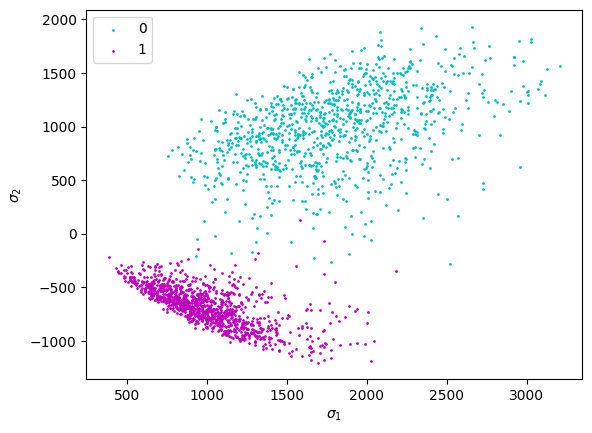
\includegraphics[scale=0.7]{mnist1.png}
      \end{center}
    \end{solution}
    \item Do this task for $k = 10$, 20, and 50. Compute $A_k = U_k \Sigma_k V_k^\top$, where $U_k$ $(V_k)$ is comprised of the first $k$ left (right) singular vectors, and $\Sigma_k = \textsf{diag}\{\sigma_1, \dots, \sigma_k\}$. Then take the first four rows of $A$ and $A_k$, reshape each of these rows back to $20 \times 20$ images, and display them.
    \begin{solution}
      This diagram and the one above were produced by \href{https://github.com/elijahkin/school/blob/main/umd/amsc660/hw3.ipynb}{this code}.
      \begin{center}
        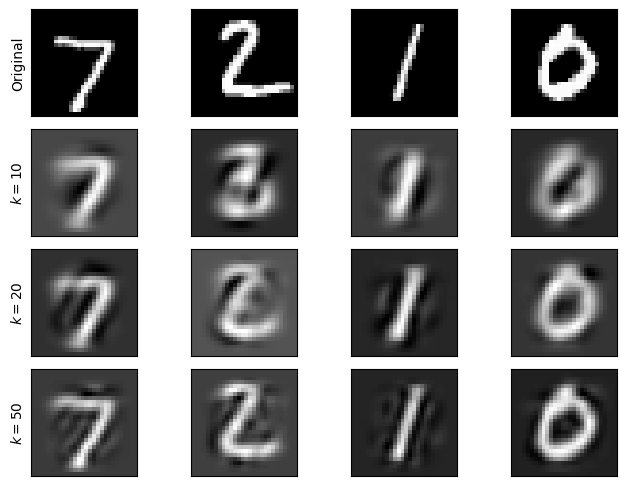
\includegraphics[scale=0.7]{mnist2.png}
      \end{center}
    \end{solution}
  \end{enumerate}
\end{questions}

\end{document}
